\hypertarget{architected\_queue}{} \section{Architected Queue in
H\-S\-A} \label{architected_queue}

H\-S\-A hardware supports kernel dispatch through user mode queues.
A queue in HSA is associated with a specific HSA component. There
are two kinds of queues that are supported, an AQL queue which can
consume any kind of packets discussed in Section~\ref{AQL}. A
service queue is defined a queue that consumes AGENT\_DISPATCH
packets. AGENT\_DISPATCH packets can be used to specify
runtime-defined or user registered functions that will be executed
on the agent (typically, the host CPU). 

An HSA component can have multiple AQL and service queues associated
with it.  Conceptually, user mode queues are ring buffers that
expose separate memory locations defining the current read and write
state of the queue. The HSA runtime allows the user to create a user
mode queue via.\ \texttt{hsa\_queue\_create} API. The same API also
allows to user to create a service queue. The user may chose to
manage their own service queue.

In a HSA system, agents write AQL packets to the user mode queue
queue to enqueue work on to the HSA components. The queue memory is
processed by HSA packet processor(s) as though it is a ring buffer.
The details on how commands can be written to the queue via AQL
packets and the structure of the AQL packet are discussed in
Section~\ref{AQL}.


A queue in HSA is defined with the following structure:

\input{STRqueue_struct}

\texttt{base\_address} is the starting address of the buffer where
the packets will be written.  \texttt{size} is simply the size of
the queue in bytes.  The \texttt{queue\-\_\-id} member is the unique
(per-process) identifier for a queue and helps identify a queue when
more than one queue is present in the system.

Internally, the queue structure contains read index and write index.
These are not exposed to the user directly. The user can access them
by using the \texttt{hsa\_queue\_get/cas/add\_write\_index} and
\texttt{hsa\_queue\_get\_read\_index} API. All of these API calls
have different versions for different memory scopes.

The API is defined as follows:

\input{APIqueue_update}

These API are all setter/getter APIs and hence do not return
\texttt{hsa\_status\_t}. If the queue structure passed to the API is
invalid, the behavior of the API is undefined. All the API return
the value of the corresponding index. The CAS, ADD and WRITE API on
the write index return the value of the write index prior to the
update.

The write index is a unique identifier for AQL packets in the
queue. The read index indicates the next AQL packet that will be
consumed by the HSA packet processor.  The write index 
memory is updated by the agents via the runtime defined 
API, while the read index memory location is updated by
the H\-S\-A Component and can be read by the agent, 
a runtime specified API call, or the kernel via HSAIL operation.

The read index is automatically advanced when a packet is
read by the HSA packet processor. When the agent observes that read
index matches write index, at that instance, the queue can be
considered empty (it does not mean that the kernels have finished
execution, just that all packets have been consumed). The write
index and the read index never wrap when the write index reaches
its maximum value. An asynchronous error is generated by the packet
processor and queue is put in error state.

The {\itshape
queue\_active\_group\_count} is the count of maximum number of
work-groups that can be executed in parallel for dispatches executed
on this queue.

The \texttt{doorbell\_signal} is a signal from the agent writing the
AQL packet to the HSA packet processor indicating that it has work
to do. The value which the \texttt{doorbell\_signal} must be
signaled with shall be the latest write index at
which an AQL packet has been written into.  The purpose of this
signal is to \emph{inform} the HSA packet processor that it has
packets that need to be processed. However, packets may be processed
by the HSA packet processor even before the
\texttt{doorbell\_signal} has been signaled by the agent writing the
AQL packet.  This is because when write index is advanced by the
agent there are two scenarios that could arise: 

\begin{itemize}
        \item the HSA packet processor is in some low-powered state
                awaiting work and requires the
                \texttt{doorbell\_signal} signal to \emph{wake} it
                to continue reading packets.
        \item the H\-S\-A
                packet processor is already actively processing a
                packet and observes the write index being
                updated by the agent and continues to process the
                new packets written -- even before the agent has
                signalled the \texttt{doorbell\_signal}. 
\end{itemize}

Hence, despite the fact that the AQL packet for which the agent is
signalling the doorbell may already have been processed, the agent
must ring the doorbell for every batch of AQL packets written. 

The \texttt{hsa\_queue} structure is the output of
\texttt{hsa\_queue\_create} function, which is defined as
follows:

\input{APIqueue_create}

The \texttt{hsa\_queue\_create} API allocates the memory for the
queue. Space for \texttt{size} number of packets is allocated by the
implementation. The size is required to be aligned with a power of
two number of AQL packets. 
The {\itshape hsa\_queue\_mailbox\_t} structure returned by the
queue create call contains {\itshape mailbox\_ptr} and {\itshape
mailbox\_signal}. Their purpose is getting execution information
when a \ttbf{debugtrap\_u32} 
HSAIL instruction is used in the user kernel. The user can wait on
the {\itshape mailbox\_signal} and process the information in the
{\itshape mailbox\_ptr} as discussed in
Section~\ref{coreapi_coredebug}. 
The pointer to the beginning of the memory allocated can be obtained
from the queue structure in the field \texttt{base\_address}.  No
memory shall be allocated by an implementation if the queue creation
fails. An implementation may or may not initialize the
\texttt{hsa\_queue} structure if queue creation fails. Hence the
user should rely on the error code to determine if the
\texttt{hsa\_queue} structure is valid. 

This service queue is configured when a user mode queue is created.
The service queue is visible to HSA agents through the queue
structure \texttt{service\_queue} field and is serviced by an
appropriate HSA agent. The application may chose to not use a
service queue, select the runtime managed service queue, or a queue
managed by the application via.\ the {\itshape
hsa\_service\_queue\_type\_t} enumeration input parameter.  Address
of the service queue associated with the user mode queue is returned
in the queue structure. If there is no associated service queue then
the NULL address will be returned.  The API allows different user
mode queues to have a different associated service queue. It also
allows for the service queue to be user managed. The API allow
allows the user to specify that runtime return a default shared
service queue which is created when the runtime is initialized. 

The \texttt{hsa\_queue\_create} API returns
\texttt{HSA\_STATUS\_SUCCESS} when the queue is successfully
created.  Otherwise, it can return one of the following status
messages:

\begin{easylist}
& \texttt{HSA\_STATUS\_ERROR\_INVALID\_ARGUMENT} error code is
returned when the queue size is not a power of two, when the error
message queue handle is invalid, or the component is not valid. This
error code is also returned when {\itshape queue} is NULL.  

& \texttt{HSA\_STATUS\_ERROR\_OUT\_OF\_RESOURCES} if there is a failure
in allocation of an internal structure required by the core runtime
library in the context of the queue creation. This error may
also occur when the core runtime library needs to spawn threads or
create internal OS-specific events. This error is also returned when
a service queue or a user mode queue cannot be allocated.
\end{easylist}

The first ratified version of the SAR specification does not define the
\texttt{queue\_type} and \texttt{queue\_feature} -- they have been
marked as fields for future expansion. 

The API to destroy a queue is defined as follows:

\input{APIqueue_destroy}

After queue destruction, it is considered undefined to access the
memory pointed to be the \texttt{base\_address} or the {\itshape
service\_queue}. 

\hypertarget{queue_inactivate}{}\subsection{ Inactivating a Queue}
\label{queue_inactivate}
The queue can forcefully be inactivated by the user. This will kill
any pending executions and prevent any new packets from being processed.
Any more packets written to the queue once it is inactivated will be
ignored by the packet processor.

The API for inactivating the queue is defined as follows:

\input{APIqueue_inactivate}

\hypertarget{queue_errors}{}\subsection{Queue Error Reporting,
Inactivation and Queue State} \label{queueerrors}
The HSA queue structure includes an error message queue, {\itshape
message\_queue\_handle}, that the user must initialize and pass as
an argument at queue creation. The error message queue may be
created by the user using the
\texttt{hsa\_error\_message\_queue\_create} API. The user may also
use the default error message queue generated by the
\texttt{hsa\_initialize} API.

There are two primary kinds of errors that impact queue
processing and render a queue inactive:
\begin{itemize}
        \item Errors due to packet processing, such as invalid
                format, field-value, invalid signal, etc.
        \item Errors occurring during subsequent resource/dispatch
                setup or system errors during dispatch.
\end{itemize}

A queue in HSA, once created, can be in one of the following states:
\emph{active}, \emph{error pending inactive}, \emph{error inactive}
or \emph{destroyed}.

\begin{description}
\item[Active] Once a queue is successfully created using the
\texttt{hsa\_queue\_create} API, it enters an active state, packets can
be put on the queue and when the write-index is updated and the
doorbell is updated, the packet processor processes the packets. The
actual initiation of dispatch may depend on the resources available
for the dispatch. 
Only in the \emph{active} state, writing packets to
the queue, updating the write index or ringing the doorbell has 
any effect. The queue is no longer being monitored by a queue packet
processor for new packets in any other state.

\item[Error pending inactive] When packet processing or
dispatch setup encounters one of the errors described above, the
queue packet processor stops packet processing. 
At this point, there might be in-flight kernels and resources (such
as segment allocation) that have been setup for a dispatch but have
not yet been freed. So the queue is not entirely inactive, but once
the asynchronous activity concludes, it will become inactive.  A
queue in \emph{error pending inactive} state is not to be considered
as destroyed, it still needs to be destroyed so the runtime can
reclaim the memory allocated for this queue. If the user provides a
callback at queue creation time, the callback is invoked after
the queue is marked inactive.

\item[Inactive] If all the asynchronous activity concludes, the
queue enters the inactive state. 
A queue can also enter this state when the user explicitly invokes
the \texttt{hsa\_queue\_force\_inactivate} API (note that the callback
implementation for the queue error callback can invoke this API).  
In an inactive state, the queue
structure and its packets may be inspected. Only the packets that
are between the read index and the write index
in the queue structure are considered to be valid for inspection by
the user. The packet processor guarantees that all the packets that
have been consumed by the packet processor (see
Section~\ref{dispatch_packet}) will be signalled with either the
completion information or an error. 
Invocation of \texttt{hsa\_queue\_force\_inactivate} API when the
queue already is in the inactive state has no effect.

\item[Destroyed] The queue has been destroyed by the user.  The
resources allocated to the queue and the memory for the queue are no
longer valid. The queue structure is no longer valid. 
\end{description}

\begin{SCfigure}
  \centering
  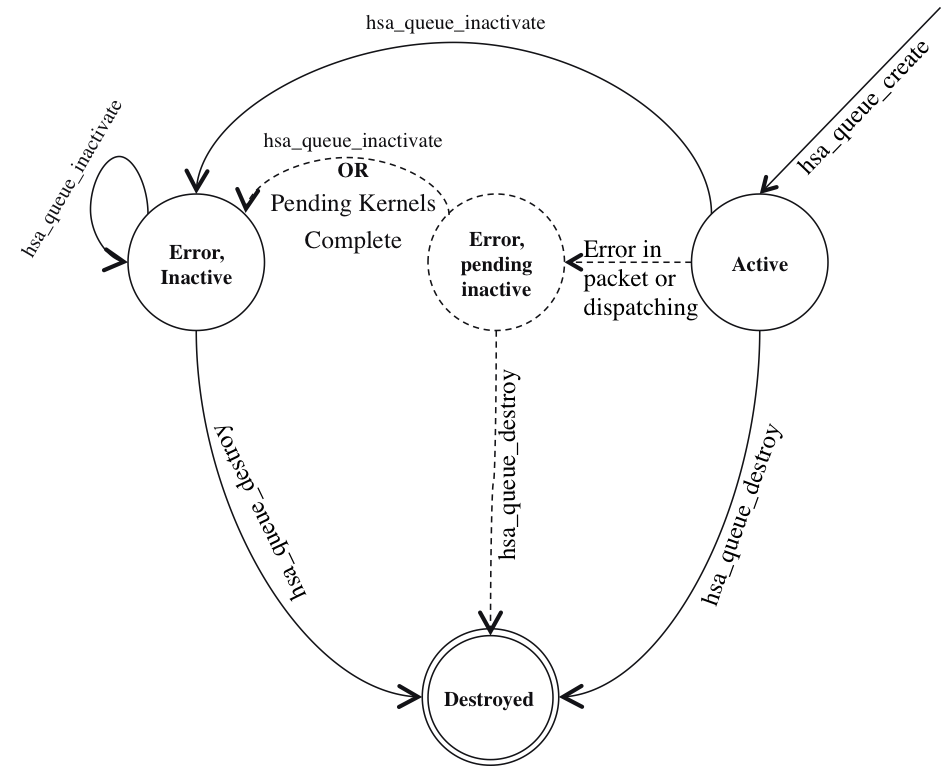
\includegraphics[width=0.5\textwidth] {queuestate}
  \centering
  \caption{Once the queue is created and is active, any error in
          packet processing takes the queue into pending inactive
          state where the queue is performing tasks to get to
          inactive state. Failure during the attempt to inactivate
          results in queue reaching an error state. A queue that is
          in active, error or inactive state may be destroyed by
          using the \texttt{hsa\_queue\_destroy} API provided by
  the HSA runtime.}
  \label{fig:queuestate}
\end{SCfigure}

A state diagram showing the various states and transitions is shown
in Figure~\ref{fig:queuestate}.

The queue will report packet processing or parsing error, system
error, dependency resolution error, and signalling error (signal
destroyed by the time it needed to be signalled by packet processor).

The queue error reporting infrastructure supports and reports a
single error per queue and attempts to inactivate the queue on the
first error it encounters.

\hypertarget{coreapi_multithreading}{}\subsection{Multi-\/\-Threaded
Queue Access}\label{coreapi_multithreading}
H\-S\-A Core API does not provide explicit API for synchronized
access to the queues -- the architected queue data structure and
read/write index update API are
sufficient to allow users to implement thread-safe packet insertion
into the queue. Users can use several techniques to support
multiple concurrent writers writing AQL packets to the queue.  The
following example code illustrates one such technique -- several
other techniques that allow concurrent writes to the queue can be
utilized in a similar way.

The sample code below demonstrates a simple reader and writer logic
to do a multi-threaded queue access using the queue structure above.

\begin{framed}
\lstinputlisting[language=C,numbers=none,commentstyle=\color{brown},keywordstyle=\color{blue}]{queue.c}
\end{framed}

